%%%
%%% Hauptdokument
%%%

\documentclass[
	a4paper,     		%% Papiergroesse: A4 OBSOLETE
	twoside,     		%% Zweiseitiges Layout (alternativ: oneside)
	headsepline, 		%% Horizontale Linie unter Kopfzeile
	footsepline, 		%% Horizontale Linie ueber Fusszeile
	titlepage,   		%% Eigenstaendige Titelseite (alternativ: notitlepage)
%	halfparskip, 		%% Halbe Leerzeile zwischen zwei Abschnitten (alternativ: parskip, ...)
	12pt,        		%% Schriftgroesse: 12pt (alternativ: 10pt, 11pt, ...) OBSOLETE
%	bibtotoc,			%% Bilbiographie in's Inhaltsverzeichnis aufnehmen
%	liststotoc,			%% Indexe in's Inhaltsverzeichnis aufnehmen
%	smallheadings,		%% Kleine Ueberschriften
%	DIV1,				%% Divisor, Zeilenlänge ca. 70 Zeichen
%	BCOR01cm,			%% Bindekorrektur
%	draft			  	%% Entwurfsmodus, volle/leere Boxen markieren
%	abstracton			%% Titel "`Zusammenfassung"' einschalten
]{scrreprt}

%%%
%%% Pakete
%%%

%%% Glossar
% \usepackage[german]{gloss}
% \newcommand{\acr}[1]{{\small\gloss[word]{#1}}}
% 
% \newcommand{\abk}[1]{#1\xdot}
% \DeclareRobustCommand\xdot{\futurelet\token\Xdot}
% \def\Xdot{\ifx\token\bgroup.\else\ifx\token\egroup.\else
%   \ifx\token\/.\else\ifx\token\ .\else\ifx\token!.\else
%   \ifx\token,.\else\ifx\token:.\else\ifx\token;.\else
%   \ifx\token?.\else\ifx\token/.\else\ifx\token'.\else
%   \ifx\token).\else\ifx\token-.\else\ifx\token+.\else
%   \ifx\token~.\else
%   \ifx\token.\else.\ \fi\fi\fi\fi\fi\fi\fi\fi\fi\fi\fi\fi\fi\fi\fi\fi} 
% \newcommand{\zB}{\mbox{z.\,B}\xdot}

%%% Literaturverzeichnis, deutschen Stil benutzen (dinat)
%%% TODO: funktioniert leider derzeit nicht mit TeXlipse!
%\usepackage[square]{natbib}
%\citestyle{dinat}

%%% Grafik
\usepackage{pstricks}

%%% UML
%\usepackage{pst-node}
%\usepackage{pst-uml}
%\let\umlClass\pstumlClass	%%% workaround: pst-uml und uml kollidieren
%\usepackage{uml}

%%% Deutsche Sprache verwenden
\usepackage{ngerman}

%%% Kodierung der Eingabezeichen setzen (fuer dt. Umlaute etc.)
%%% Für Linux: [latin1] für Windows: [ansinew]
\usepackage[utf8]{inputenc}

%%% Zeichen-Kodierung in PDF-Dokumenten
\usepackage[T1]{fontenc}
%\usepackage{ae,aecompl}

%%% Web-Addressen auch mit T1-Encoding
\usepackage[T1]{url}
%%% ... und in tt-Font
\urlstyle{tt}

%%% amsmath, amssymb, amstext: Unterstuetzung div. mathematischer Zeichen etc.
\usepackage{amsmath,amssymb,amstext}

%%% pifont: "pifont Xs and Check Marks"
% \usepackage{pifont}

%%% PostScript-Fonts ersetzen
\usepackage{psfrag}

%%% Programmcode einbinden, Listings
\usepackage{listings}

%%% Farb-Unterstuetzung
\usepackage{color}

%%% Tabellen
\usepackage{booktabs}
\usepackage{array}
\usepackage{multirow}
\usepackage{tabularx}
\usepackage{threeparttable}	% Fussnoten in table-Umgebung

%%% Floats strikter positionieren (Option 'H'ere)
\usepackage{float}

%%%
%%% Pakete konfigurieren, Definitionen
%%%

%%% Ueberschriften bis zur Ebene 3 nummerieren
\setcounter{secnumdepth}{3}

\setcounter{tocdepth}{3}

%%% Neue Spaltentypen definieren
\newcolumntype{N}{>{\bfseries\scriptsize}l}
\newcolumntype{V}[1]{
	>{\bfseries\scriptsize\raggedright\hspace{0pt}}p{#1}
}

%%% Ein paar Farbdefinitionen (s. http://texnik.de/listings/listing0.pdf)
\definecolor{hellgelb}{rgb}{1,1,0.8}
\definecolor{hellgrau}{rgb}{0.95,0.95,0.95}
\definecolor{colKeys}{rgb}{0,0,1}
\definecolor{colIdentifier}{rgb}{0,0,0}
\definecolor{colComments}{rgb}{1,0,0}
\definecolor{colString}{rgb}{0,0.5,0}

%%% Konfiguration des listing-Paketes
\lstset{%
	float=hbp,%
	basicstyle=\ttfamily\footnotesize, %
	identifierstyle=\color{colIdentifier}, %
	keywordstyle=\color{colKeys}, %
	stringstyle=\color{colString}, %
	commentstyle=\color{colComments}, %
	columns=flexible, %
	tabsize=4, %
	frame=tb, %
	extendedchars=true, %
	showspaces=false, %
	showstringspaces=false, % 
	numbers=left, %
	numberstyle=\tiny, %
	breaklines=true, %
	backgroundcolor=\color{hellgrau}, %
	breakautoindent=true, %
	captionpos=b%,
	language=XML,%
	aboveskip=\bigskipamount,%
	belowskip=\medskipamount,%
}

%%% Benoetigte Sprachen laden
%\lstloadlanguages{XML,XSLT,SQL,HTML,PHP,XQuery}

%%%
%%% Seitenlayout, Schriften
%%%

%%% scrpage2: KOMA Kopf- und Fusszeile
\usepackage[automark]{scrpage2}

%%% KOMA-Script: Optionen
% \KOMAoptions{fontsize=12pt}
% \KOMAoptions{paper=a4}

%%% EM unterstrichen darstellen
%\usepackage{ulem}

%%% Schrift fuer Captions verkleinern
\setkomafont{captionlabel}{\scriptsize}
\setkomafont{caption}{\usekomafont{captionlabel}}

%%% Schrift fuer Ueberschriften umstellen
%\setkomafont{sectioning}{\normalcolor\bfseries}

%%% Schriften fuer Titel- und Fusszeile umstellen
%\setkomafont{pagehead}{\normalfont\sffamily}
\setkomafont{pagenumber}{\normalfont\rmfamily\slshape}

%%% Part-Ueberschrift nicht fett drucken
%\addtokomafont{part}{\mdseries}
%\addtokomafont{partnumber}{\mdseries}

%%% Default-Platzierungsbeschraenkungen aendern,
%%% s. http://www.dante.de/faq/de-tex-faq/html/makros2.html#1
% \makeatletter
% 	\renewcommand{\fps@figure}{htbp}
% 	\renewcommand{\fps@table}{htbp}
% \makeatother

%%%
%%% PDF-Einstellungen
%%%

%%% Fallunterscheidung: PDF- oder 'normale' Erstellung?
\usepackage{ifpdf}

%%% Falls wir PDF erzeugen...
\ifpdf
  %%% Serifenlose Schriften benutzen
  \usepackage{mathpazo}
  \usepackage[scaled=.95]{helvet}
  \usepackage{courier}	
  \renewcommand{\familydefault}{\sfdefault}
  \usepackage[sf]{titlesec}

  %%% Unterstuetzung fuer Grafiken
  \usepackage[pdftex]{graphicx}
 
  %%% Kompressionslevel: 0-9
  \pdfcompresslevel=9

  %%% Hyperlinks in PDF-Dokumenten
  \usepackage[%
  	pdftex,
    pagebackref=false,			%% Seitenzahlen der Quellseite(n) in Bibliographie auflisten? (true|false) 
    colorlinks=true,				%% Farblinks? (true -> Screen | false -> Print)    
    %%% PDF-spezifische Optionen
    bookmarks=true,					%% PDF-Bookmarks erstellen? (true|false)
    bookmarksopen=true,			%% Anfangs alle Bookmarks ausgeklappt anzeigen? (true|false) 
    bookmarksnumbered=true,	%% Abschnitt-Nummerierung in Bookmarks integrieren? (true|false)
    pdfstartpage={1},				%% Startseite beim Oeffnen der Datei
    pdfpagemode=UseOutlines,%% Anzeigemodus? (None|UseOutlines|UseThumbs|FullScreen)
    a4paper=true,						%% A4-Format
    breaklinks=false,
    linkcolor=gray					%% Link-Farbe
  ]{hyperref}

	%%% Dateiendung fuer Grafiken setzen -- so kann beim Einbinden der Grafik
	%%% auf die Endung verzichtet werden und es wird automatisch die korrekte 
	%%% Datei ausgewaehlt (.eps / .pdf)
  \DeclareGraphicsExtensions{.pdf}
  
  %%% Pfad fuer Bilder setzen
  \graphicspath{{../images}}

%%% ... oder im 'normalen' Modus sind
\else

  %%% Unterstuetzung fuer Grafiken
  \usepackage[dvips]{graphicx}

  %%% s.o.
  \DeclareGraphicsExtensions{.eps}
  \graphicspath{{../images}}

  %%% Hyperlinks in PS-Dokumenten, Optionen s.o.
  \usepackage[%
    dvips,
    colorlinks=false,
    breaklinks=true,				%% Duerfen Links umbrochen werden? (true|false)
  ]{hyperref}

\fi

%%% Informationen ueber das PDF-Dokument setzen
\hypersetup{
  pdftitle={Lernfähige autonome Roboter},%
  pdfauthor={Jan Tammen (jan.tammen@htwg-konstanz.de),%
  			 Kornelius Nägele (knaegele@htwg-konstanz.de),%
  			 Christian Kungel (christian.kungel@htwg-konstanz.de)},%
  pdfsubject={Robotik},%
  pdfcreator={Jan Tammen (jan.tammen@htwg-konstanz.de)},%
  pdfproducer={LaTeX with pdfeTeX},%
  pdfkeywords={Robotik, Lernfähige autonome Roboter, Reinforcement Learning, Q-Learning, Monte Carlo},
  % pdfpagelayout=TwoColumnRight,
  pdffitwindow=true,
%  pdfstartview=FitH,
}

%%% Links im dvips-Mode auch umbrechen
\usepackage{breakurl}

%%%
%%% Layout der Titelseite
%%%

%%% Titelkopf, erscheint oberhalb des Titels
\titlehead{
	\begin{figure}[H]
		\centering
		
\includegraphics[width=\textwidth]{../images/htwg-logo}
	\end{figure}
}

%%%% Subject, erscheint oberhalb des Titels
\subject{Seminar Robotik WS 06/07}

%%% Titel
\title{Lernfähige autonome Roboter}


%%% Publisher, hier: Verantwortlicher Prof.
\publishers{%
	\small
  Prof.\,Dr.\,Bittel, Fakultät Informatik, HTWG Konstanz
}

%%%% Autor. Weitere Autoren mit \and{<Name>} hinzufuegen
\author{%
	Christian Kungel
	\and{%
		Kornelius Nägele
	}%
	\and{%
		Jan Tammen
	}%
}%

%%% Datum setzen
\date{\today}

%%% Rueckseite der Titelseite
\lowertitleback{%
	\footnotesize%
	Erstellt mit \LaTeXe\ unter Verwendung des \KOMAScript-Pakets.
}

%%%
%%% Header und Footer
%%%

\pagestyle{scrheadings}

%%% Kopfzeile in den Rand ragen lassen
%\setheadwidth{textwithmarginpar}

%%% Fusszeile in den Rand ragen lassen
%\setfootwidth{head}

%%% \automark[rechte Seite]{linke Seite}
%\automark[subsection]{section}

%% Header links -- section
%\ihead[]{\rightmark}

%% Header rechts -- chapter
%\ohead[]{\leftmark}

%% Header mittig -- leer
\chead[]{}

%% Footer mittig -- leer
\cfoot[]{}

%% Footer rechts -- Seitenzahl
\ofoot[]{\thepage}

%%% Footer links -- Titel der Arbeit
\ifoot[]{\footnotesize{Lernfähige autonome Roboter}}

%%%
%%% Sonstiges
%%%

%%% Glossar und Index erstellen 
% \makegloss
% \makeindex

%%%
%%% Beginn Hauptdokument
%%%
\begin{document}

%%% Titelseite erstellen
\maketitle

%%% Inhaltsverzeichnis erstellen
%\newpage
\tableofcontents

%%% Bildverzeichnis erstellen
%\newpage
%\listoffigures

%%% Tabellenverzeichnis erstellen
%\newpage
%\listoftables

%%%
%%% Beginn Inhalt
%%%
%%% Inkludieren Kapitel 1
\chapter{Einleitung}
\section{Was heißt Lernen?}
Die Psychologie bezeichnet jede Interaktion des Menschen mit seiner Umwelt - 
zum Beispiel die Reaktion auf Reize - als Verhalten. Jeder Mensch verfügt zu 
einem bestimmten Zeitpunkt seines Lebens über ein bestimmtes Repertoire von 
Verhaltensmöglichkeiten. Dieses Repertoire ändert sich im Laufe der Zeit. 
Liegen die Gründe für diese Änderung in äußeren Einwirkungen und nicht in der 
Biologie (Alterungsprozess), so spricht man von Lernen. Daraus folgt die 
folgende Definition:

\begin{quotation}
Lernen ist eine dauerhafte (im Gegensatz zu einer vorübergehenden) Änderung
des Verhaltens und von Verhaltenspotenzialen, die durch Übung (im Gegensatz etwa
zu Reifung, Prägung oder Krankheit) erfolgt.
\end{quotation}

\section{Was heißt Maschinelles Lernen?}
Der psychologischen Definition des Lernens stellen wir nun zwei Definitionen
des Maschinellen Lernens (engl. Machine Learning) gegenüber:

\begin{quotation}
Machine Learning is programming computers to optimize a performance
criterion using example data or past experience \cite{Alpaydin2004}.
\end{quotation}

\begin{quotation}
A computer program is said to learn from experience $E$ with respect to some 
class of tasks $T$ and performance measure $P$, if its performance at tasks in 
$T$, as measured by $P$, improves with experience $E$ \cite{Mitchell1997}.
\end{quotation}

\section{Arten des Maschinellen Lernens}
Hier unterteilt man die Lernmethodiken in drei hierarchisch übergeordnete
Klassen, sogenannte Problemklassen. 
\par Zum einen die Klasse des \textbf{"`Supervised Learnings"'}, die darauf
abzielt, dass bei allen Beispielen Kennzeichungen gegeben sind und hieraus ein 
Zusammenhang zwischen den Beschreibungen der Beispiele und ihren Kennzeichnungen
ermittelt werden soll. \par Die zweite Problemklasse stellt das sogenannte
\textbf{"`Unsupervised Learning"'} dar. Dabei sind zu den Beispielen keine Kennzeichungen gegeben. 
\par Die letzte und dritte Klasse dieser Lernverfahren ist die Art des
\textbf{"`Reinforcement Learnings"'}, die Gegenstand und Schwerpunkt des
nächsten Kapitel sein wird.

%%% Inkludieren Kapitel 2
\chapter{Reinforcement Learning}
\section{Grundlegende Techniken}
Die Techniken, die im Bereich der nicht-photorealistischen Computergrafik 
eingesetzt werden, lassen sich in 3 Kategorien unterteilen:
\begin{itemize}
  \item im Geometrieraum
  \item im Projektionsraum
  \item im Bildraum.
\end{itemize}
  Im Geometrieraum wird das 3D-Modell der nachzubildenden Realität erzeugt, 
  dieses Modell wird dann über einen Betrachterblickpunkt in den 2D-Bildraum 
  projiziert. NPR-Techniken können in jeder der 3 Ebenen eingesetzt werden.

\subsection{Techniken im Geometrieraum}
Diese Art von Techniken übt direkten Einfluss auf die 3D-Geometrie eines Objektes 
aus. Nachteil dieser Technik ist jedoch der hohe Zeitaufwand bei der 
Manipulation und daher kommen diese Verfahren praktisch eher selten zum 
Einsatz. Techniken dieser Klasse sind zum einen "`Computer Sketching"', "`Noise 
Modifier"' und "`Level of Detail"'. Die Funktionsweise dieser Methoden wird im 
Nachfolgenden kurz vorgestellt.

\subsubsection{Computer Sketching}
Das "`Computer Sketching"' Verfahren wurde 1990 von Paul Bourk entwickelt. Er 
stellte sich die Frage, ob CAD-Anwendungen auch unscharfe, an menschliche 
Skizzen erinnernde Entwürfe ausgeben können. Dabei legte er folgende Kriterien 
für Skizzen fest: In Skizzen enden Linien nicht exakt an Kreuzungen 
(Schnittpunkten), sondern gehen über diese hinaus. Außerdem sind Linien nicht 
gradlinig sondern „verwackelt“. Diese Effekte erreichte Bourk durch die 
Manipulation des 3D-Modells, Linien wurden um einen zufälligen Faktor 
verlängert, gespalten und einer Mittelpunktverschiebung unterworfen.
\begin{figure}
  \centering
  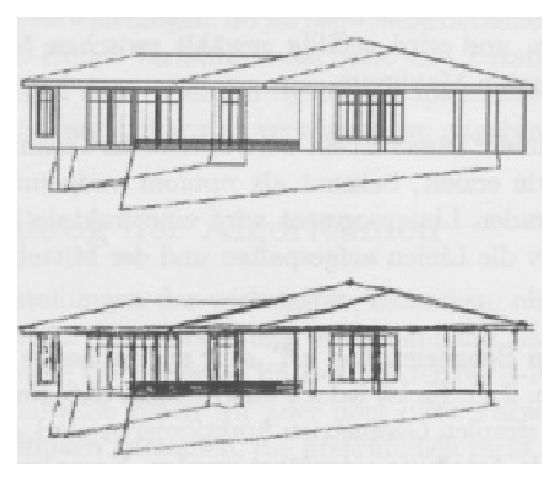
\includegraphics[width=0.60\textwidth]{../images/ComputerSketching}
  \caption{Oben Ausgabe ohne Computer Sketching, unten Ausgabe in der
  "`Sketchy"' Variante}
  \label{fig:ComputerSketching}
\end{figure}

\subsubsection{Noise Modifier}
In einer weiteren Technik im Geometrieraum kommen sogenannte Noise-Modifier zum 
Einsatz, diese erzeugen ein "`Rauschen"' in den 3D-Modellen. Dieses "`Rauschen"' 
wird erreicht, indem die Geometriepunkte der Flächen des Modells um einen 
zufälligen Faktor verschoben werden. Diese Verfahren finden hauptsächlich 
Anwendung auf glatte Flächen, um "`natürliche"' Flächen zu erzeugen.

\subsubsection{Level of Detail}
Ein Verfahren, das in vielen Bereichen Verwendung findet, ist das Level of 
Detail Prinzip, das unterschiedliche Detailstufen zur Darstellung nutzt. Es 
wird unter anderem in der Kartographie eingesetzt. Hier wird die Detailstufe in 
Abhängigkeit vom Maßstab der Karte dargestellt. Ein weiterer Einsatzbereich ist 
die photorealistische Computergrafik. Hier erfolgt die Darstellung der Details 
in Abhängigkeit von der Betrachterposition. Je näher ein Objekt dem Betrachter 
ist, desto genauer wird es dargestellt. NPR modifiziert dieses Prinzip und 
setzt die Detaillevel in Abhängigkeit zur "`Wichtigkeit"' der einzelnen Objekte. 
Je wichtiger ein Objekt für die Darstellung ist, desto genauer wird es 
dargestellt. Eine Möglichkeit zur Umsetzung bietet die Meshsimplifizierung. 
Hierbei wird die Anzahl der Polygone eines "`unwichtigen"' 3D-Modells reduziert 
und die äußere Form approximiert. Diese Technik unterstützt eine schnelle 
Verarbeitung und bietet so einen Einsatz in Echtzeitsystemen.

\subsection{Techniken im Projektionsraum}
Techniken im Projektionsraum werden meist mit Bildraumverfahren kombiniert, um 
ein leichteres Arbeiten mit 3D-Modellen und eine Erhöhung der grafischen 
Qualität der Ausgabe zu ermöglichen. Die Techniken arbeiten nach der Projektion 
und nutzen zusätzliche 3D-Informationen, wie Z-Werte oder Flächennormalen. 
Ein großer Vorteil dieser Techniken ist, wie oben schon angesprochen, die 
leichte Handhabung mit 3D-Modellen und daraus resultierend, die Erhöhung der
grafischen Qualität der Ausgabe. Ein Nachteil ist die komplizierte Berechnung
aufgrund der Verzerrungen. Verfahren, die im Projektionsraum Anwendung finden,
sind G-Buffer, Line-Rendering und Stroke Textures-Verfahren.

\subsubsection{G-Buffer}
Der G-Buffer (Saito u.\ Takahashi, 1990), ausgeschrieben "`Geometrie-Buffer"' 
genannt, ist in den meisten kommerziellen Cartoon-Render-Paketen implementiert. 
Das Prinzip basiert auf einer zusätzlichen Speicherung von geometrischen Daten 
zur Informationsgewinnung im Bildraum. So ist es beispielsweise möglich die 
Flächennormalen, die UV-Koordinaten oder die Z-Buffer-Werte eines 3D-Modells 
zusätzlich zu speichern, dies geschieht im Projektionsraum. Die Informationen 
werden dann für die Bilderzeugung aus dem G-Buffer extrahiert, analysiert und 
zusammengefügt.

\subsubsection{Line-Rendering}
Mit Hilfe der Line-Rendering Methode wird die Semantik von Linien simuliert. 
Dabei wird zwischen geometrischer und stilistischer Semantik unterschieden. 
Unter geometrische Semantik fallen Begrenzungen, Silhouetten, Diskontinuitäten 
und isoparametrische Konturen. Linienstärke, Transparenz und Linientyp 
(gestrichelt, durchgezogen, etc.) hingegen machen die stilistische Semantik 
aus. Im Projektionsraum werden für jede Linie die Charakteristiken, wie 
Wichtigkeit, Linientyp und Verdeckung, zum Beispiel mit Hilfe von 
Inferenzregeln bestimmt. Dann werden diese Attribute in geeigneter Form, etwa 
in Matrixform, abgespeichert und zur Bilderzeugung genutzt. Da sich diese 
Technik primär mit Linienstilen und ihren Semantiken beschäftigt, bietet sie 
eine gute Kombinationsmöglichkeit mit anderen NPR-Techniken, wie etwa mit dem 
zuvor vorgestelltem G-Buffer-Verfahren.

\subsubsection{Stroke Textures}
Das Prinzip der Stroke Textures (Winkenbach \& Salesin, 1994) basiert auf 
konventionellen 2D-Malsystemen. Es wird eine "`strichbasierte"' Textur 
angefertigt, die mittels Texturemapping auf bereits projizierte 3D-Objekte 
aufgebracht wird. Hierbei ist eine Anwendung des LOD-Prinzips auf die Textur 
möglich. Der Benutzer ist in der Lage die Linienstärke sowie sogenannte 
"`Detail Tags"' zu spezifizieren, um eine genauere Darstellung der Textur an 
ausgewählten Stellen zu erreichen.

\subsection{Techniken im Bildraum}
Bei Techniken im Bildraum geht man von einem vorhandenen Bild aus, das 
analysiert und neu "`gezeichnet"' wird. Vorteilhaft ist hierbei, dass das Bild 
bereits vorhanden ist, also keine Viewing-Pipeline nötig ist. Ein tragender 
Nachteil der Verfahren ist der, dass im Bildraum nur ungenauere Berechnungen 
möglich sind. Einige Verfahren, die im Bildraum angewendet werden, sind Texture 
Elements, Hairy Brushes und das Iterated Funktion System.

\subsubsection{Texture Elements}
Textur Elements (Mezei et al\., 1974) wurden ursprünglich zur Synthese sehr 
"`naturalistischer"' Bilder eingesetzt, da man in Beobachtungen festgestellt 
hatte, dass in der Natur sich wiederholende Muster vorkommen. Hierbei werden 
grafische Subelemente (größer als ein Pixel), die sogenannten "`Texture 
Elements"', vorgefertigt. Diese Elemente werden dann im eigentlichen 
Bilderzeugungsprozess zusammengefügt und ergeben so das neue Bild. Um 
Variationen im Bild zu erreichen, werden Skalierungen, Rotationen und andere 
Verzerrungen auf die Texture Elements angewendet. So werden Verallgemeinerungen 
der Oberflächeneigenschaften erzielt, die wie menschliche Illustrationen wirken.

\subsubsection{Hairy Brushes}
Mit dem Verfahren Hairy Brushes versuchte Strassmann 1986 als einer der ersten 
das Verhalten von Pinsel und Farbe zu simulieren. Der Pinsel wird dabei als 
1D-Abdruck seiner Borsten implementiert. Diese Borsten laufen an einer 
parametrisierten Kurve entlang, die durch Knoten definiert ist. Jeder dieser 
Knoten enthält Informationen über Position und Druck des Pinsels. Der Druck 
wird zwischen den Knoten interpoliert und gibt an, wie viel Farbe der Pinsel an 
den Zeichenuntergrund abgibt. Jeder "`Strich"' wird mit einer speziellen Menge 
an Farbe gezeichnet, die mit zunehmender Länge des "`Striches"' abnimmt. Die 
Farbe kann durch ein "`Eintunken"' des Pinsels wieder aufgefüllt werden, dies 
ermöglicht auch Variationen in der Farbe.

\subsubsection{Iterated Function System (IFS)}
Iterated Function System beschreibt ein System von Funktionen die wiederholt 
ausgeführt werden. Das System wird vor allem zur Beschreibung von Fraktalen 
eingesetzt. Fraktale sind selbstähnlich, d.\,h\. sie sind rekursiv aufgebaut. 
Eines der bekanntesten Beispiele ist der Barnsley-Farn. Der Rekursive Aufbau 
ist besonders gut in den Farnblättern zu erkennen (siehe Abbildung 
\ref{fig:BarnsleyFarn} und Abbildung \ref{fig:BarnsleyFarnDetail}).

\begin{figure}
  \centering
  \subfloat[Barnsley Farn]{
    
\includegraphics[width=0.3\textwidth]{../images/BarnsleyFarn.eps}
    \label{fig:BarnsleyFarn}
  }
  \qquad
  \subfloat[Barnsley Farn Detailansicht]{
    
\includegraphics[width=0.3\textwidth]{../images/BarnsleyFarnDetail.eps}
    \label{fig:BarnsleyFarnDetail}
  }
\end{figure}

Barnsley nutzte das Prinzip des IFS 1988 zur fraktalen Kompression von Bildern. 
Diese Kompressionstechnik basiert auf der Selbstähnlichkeit von Bildern, dem 
sogenannten "`Collage Theorem"'. Zwischen größeren und kleineren Teilen eines 
Bildes lassen sich bestimmte Ähnlichkeiten finden. Das zu komprimierende Bild 
(\ref{fig:IFS_Lena}) wird hierbei in "`range blocks"' unterteilt, dabei ist 
eine gleichmäßige Aufteilung möglich, wobei jeder Block im Allgemeinen eine 
Größe von 8x8 Pixeln besitzt. Aber auch eine Quadtree-Unterteilung ist denkbar, 
um Details besser wiedergeben zu können. (siehe Abbildung \ref{fig:Quadtree_Lena})

\begin{figure}
  \centering
  \subfloat[Lena]{
    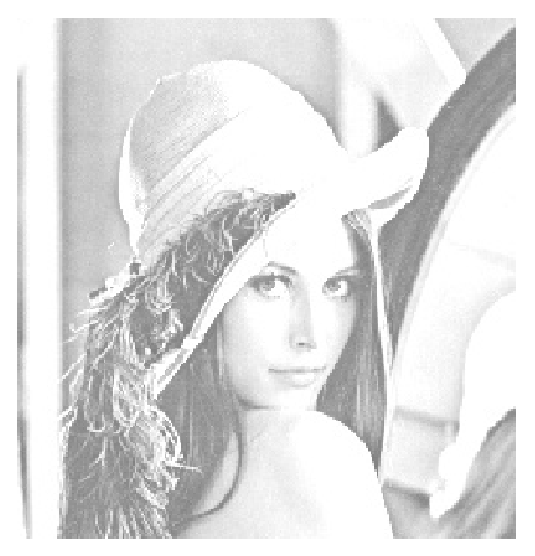
\includegraphics[width=0.4\textwidth]{../images/IFS_Lena.eps}
    \label{fig:IFS_Lena}
  }
  \qquad
  \subfloat[Quadtree-Unterteilung]{
    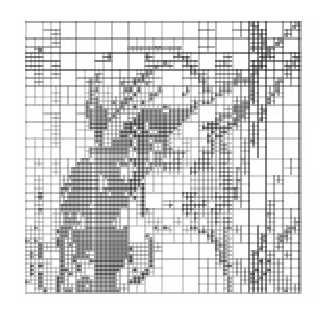
\includegraphics[width=0.45\textwidth]{../images/Quadtree_Lena.eps}
    \label{fig:Quadtree_Lena}
  }
\end{figure}

%%% Inkludieren Neuronale Netze
\chapter{Neuronale Netze}
\section{Neuronale Netze}
	\subsection{Einführung}
		\begin{frame}
			\frametitle{Einführung}

			\begin{itemize}
		      \item große Menge an vernetzten Neuronen
		      \item Gewichte an den Kanten simulieren selektive Weitergabe von echten
		      Neuronen
		      \item mehrere Schichten:
		      	\begin{itemize}
		            \item Eingabeschicht, mit allen Eingangsparamtern verbunden
		            \item verdeckte Schicht(en), mit Ausgängen der Eingabeschicht verbunden
		            \item Ausgabeschicht, mit Ausgängen der verdeckten Schicht verbunden
		          \end{itemize}
		    \end{itemize}
		\end{frame}

	\subsection{Bedeutung für Reinforcement Learning}

		\begin{frame}
	    \frametitle{Bedeutung für Reinforcement Learning}
	    Abbildung der Q-Funktion als Neuronales Netz
		  \begin{center}
			  \pgfimage[width=0.75\textwidth]{../images/rl-neuronales-netz}
		  \end{center}
	    \end{frame}

%%% Inkludieren RoboCup-Kapttel
\chapter{Das RoboCup-Projekt}
\section{Einleitung}
Das RoboCup-Projekt ist ein internationales Forschungs- und Bildungsprojekt. 
Ziel ist die Förderung der Erforschung künstlicher Intelligenz und 
Robotertechnik in einem konkreten Anwendungsumfeld: dem kooperativen 
Fußballspiel.
Dazu wird regelmäßig der \textbf{RoboCup} ausgetragen, eine Konferenz- und
Wettbewerbsveranstaltung, auf welcher diverse Wettkämpfe in verschiedenen Ligen
ausgetragen werden:

\begin{itemize}
  \item Simulationsliga (2D und neuerdings auch 3D)
  \item Small-Size-Liga
  \item Middle-Size-Liga
  \item Four-Legged-Liga
  \item Humanoid-Liga
  \item E-Liga
\end{itemize}

Mit dem RoboCupRescue-Projekt wird ein weiteres interessantes
Anwendungsfeld erschlossen: Die Suche und Rettung von Unfallopfern in unbekannten
Umgebungen durch kooperierende, mobile autonome Roboter.

\section{Das "`Mindstormers Tribots"' RoboCup-Team}
Ursprünglich entwickelt an der Universität Dortmund, ist das Team der 
"`Mindstormers Tribots"' heute am Institute of Cognitive Science an der 
Universität Osnabrück beherbergt. Neben einer Robotermannschaft der 
Middle-Size-Liga wird auch ein Simulationsteam betrieben. In den letzten Jahren 
konnten durch das Team diverse Wettbewerbserfolge erzielt werden, zuletzt 
erreichte das Middle-Size-Team im Jahr 2006 den Weltmeistertitel beim RoboCup 
in Bremen \cite{url:Neuroinformatics2006}.

In den folgenden Abschnitten werden die einzelnen Vorgehensweisen - 
insbesondere in Bezug auf das Training der Roboter - der Verantwortlichen 
sowohl in der Simulations- also auch in der Middle-Size-Liga vorgestellt.

\subsection{Simulationsliga (Brainstormers)}
In der Simulationsliga spielen zwei Teams mit jeweils elf virtuellen Agenten 
gegeneinander. Bei dieser Disziplin steht die Kooperation und Kommunikation 
unter den einzelnen Spieler-Instanzen besonders im Vordergrund. Zielsetzung ist 
die Übertragung der aus diesen Aspekten gewonnenen Erkenntnissen auf humanoide 
Roboter.
Um faire Wettbewerbsbedingungen zu garantieren, sind durch das entsprechende 
Komitee Regeln definiert, die sich im Prinzip an den FIFA-Fußballregeln 
orientieren.

\subsubsection{Funktionsweise der Simulation}
Die Simulation wird mittels einer Client-Server-Architektur realisiert. Der 
Server (offizielle Implementierung ist der \glq{}RoboCup Soccer Simulator\grq{} 
\footnote{\url{http://sserver.sourceforge.net}}) stellt dabei die Spielumgebung 
bereit und versorgt die einzelnen Clients mit (i.\,A.\ recht verrauschten) 
Sensorinformationen. Ein Client ist ein einzelner Spieler und wird durch einen 
separaten Prozess bzw.\ Thread realisiert. Clients können Aktionsbefehle an den 
Server senden und über diesen auch indirekt mit ihren Teammitgliedern 
kommunizieren.

Dies stellt bereits eine erste Einschränkung dar: Jegliche Kommunikation muss 
über den Server abgewickelt werden, wobei die Bandbreite des 
Kommunikationskanals beschränkt ist und somit nur ein sehr unvollständiger 
Informationsaustausch möglich ist.  Neben den Aktionsbefehlen (darunter z.\,B.\ 
\textsl{turn()}, \textsl{dash()} oder \textsl{kick()}) die der Server 
interpretiert, werden auch Umwelteinflüsse wie Reibung durch Boden und Wind 
sowie die Kondition der Spieler simuliert.
Die Simulation verläuft in Echtzeit - in einem Intervall von 100\,ms können die 
Clients eine Aktion durchführen und erhalten Sensorinformationen vom Server. 
Ein komplettes Spiel dauert 6000 Zyklen, was einer realen Zeit von 10\,Min. 
entspricht. Über eine sog.\ Monitor-Anwendung kann das Spielgeschehen 
visualisiert und live bzw.\ als Wiederholung verfolgt werden. Eine 
beispielhafte Spielszene ist in Abbildung \ref{fig:robocup-simulation-monitor} 
dargestellt.

\begin{figure}
  \centering
  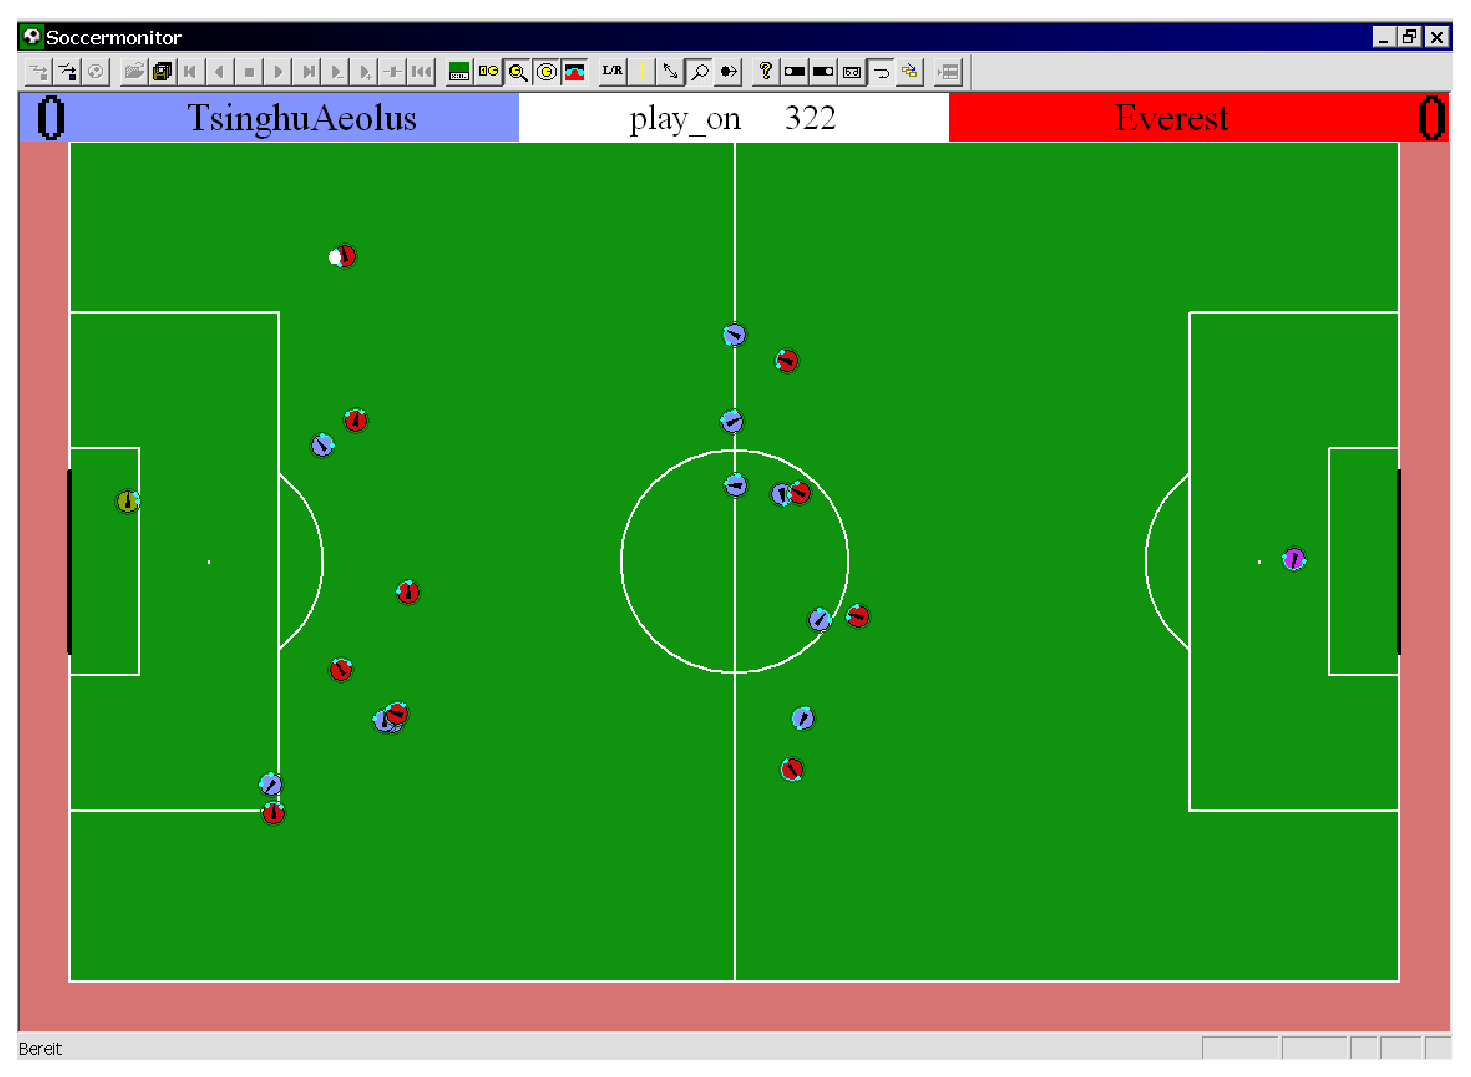
\includegraphics[width=0.80\textwidth]{../images/rcssmonitor_classic}
  \caption{RoboCup-Monitor: Visualisierung eines Spieles}
  \label{fig:robocup-simulation-monitor}
\end{figure}

Zusammenfassend ergeben sich bei der Simulation die folgenden Herausforderungen:

\begin{itemize}
  \item Aus den je 6000 Einzelentscheidungen eines jeden Spielers muss ein
  möglichst erfolgreiches, kooperatives Spiel entstehen.
  \item Sensorinformationen sind nur eingeschränkt und verrauscht verfügbar.
  \item Störungen bei Aktionsausführungen.
  \item Begrenzte Kondition der Spieler.
\end{itemize}

\subsubsection{Lernen von Einzelfähigkeiten}
Eines der allgemeinen Entwurfsprinzipien des Mindstormers-Teams ist die
Koexistenz und Austauschbarkeit von gelernten und ausprogrammierten
Verhaltensmodulen. Auf diese Weise können für einzelne Aufgaben jeweils 
verschiedenen Verfahren oder Strategien getestet und angewandt werden 
\cite{Riedmiller2006}.

Eine \textbf{Einzelfähigkeit} bezeichnet eine elementare technische Fähigkeit
eines einzelnen Spielers, die eine klar definierte Aufgabe zu erfüllen hat.
Beispiele dafür sind:

\begin{itemize}
  \item schnelles Abfangen eines rollenden Balles,
  \item effizientes Laufen zu einer Zielposition,
  \item Schießen des Balles mit spezifizierter Richtung und Geschwindigkeit,
  \item Ballhalten,
  \item Dribbeln.
\end{itemize}

Diese Einzelfähigkeiten werden aus sog.\ \textbf{Elementaraktionen} (z.B.
\textsl{dash()}, \textsl{turn()} oder \textsl{kick()}) zusammengefügt und
überführen den aktuellen Zustand in einen Zielzustand. Das Lernen einer
Einzelfähigkeit stellt nun ein dynamisches Optimierungsproblem dar, bei welchem
der Lernalgorithmus eine Strategie mit den minimalen Kosten für alle
Startzustände finden soll. Der Ablauf des Training stellt sich wie folgt dar:

\begin{enumerate}
  \item Auswahl einer Elementaraktion mit möglichst geringen Kosten.
  \item Bei Erreichen eines positiven Zielzustands: Ende der Lernsequenz
  \textsl{ohne} Kosten.
  \item Bei Erreichen eines negativen Zielzustands: Bestrafung durch hohe Kosten.
\end{enumerate}

Dieser Trainingsprozess erfolgt nun auf Episodenbasis. Ausgehend von einem
zufälligen Startzustand wählt der Spieler eine Elementaraktion - bei
Exploration eine zufällige, ansonsten diejenige mit den niedrigsten zu
erwartenden Kosten. Da das vom Server simulierte Umgebungsmodell bekannt ist,
kann der Spieler nun für alle Aktionen die Werte der Folgezustände berechnen,
was ihn befähigt, die für ihn günstigste Aktion auszuwählen. Wurde die Aktion
durchgeführt und die Kosten an den Spieler vergeben, wird die Wertfunkion
entsprechend aktualisiert.

\subsubsection{Lernen von Teamfähigkeiten}
Beim Lernen von Teamfähigkeiten ergibt sich das Problem, dass die Aktionsmenge
eines einzelnen Spielers exponentiell mit der Anzahl der Spieler anwächst,
außerdem steigt die Dimension des Zustandsvektors linear. Da aufgrund
dieser Probleme keine tatsächliche Teaminteraktion trainiert werden kann, führt
der Agent sog.\ Makroaktionen, also Kombinationen von zuvor gelernten
Einzelfähigkeiten, aus.

Um die Spieler zu einem kooperativen Spiel zu zwingen, erhalten sie alle 
dasselbe Reinforcement-Signal: das Erzielen eines Tors wird mit Nullkosten 
belohnt, das Verlieren des Balls mit Kosten von 1 bestraft. Tritt keines dieser 
beiden Ereignisse auf, so werden kleine konstante Kosten berechnet. Durch diese 
Modellierung geht jedoch nicht das Individualspiel eines einzelnen Spielers 
verloren, denn schließlich befindet sich jeder Spieler in einer anderen 
Situation und muss dementsprechend andere Aktionen ausführen. Die 
Entscheidungsfindung zur Auswahl einer Aktion läuft folgendermaßen ab:

\begin{enumerate}
  \item Alle Aktionen werden auf ihren möglichen Erfolg geprüft.
  \item Für alle erfolgreichen Aktionen wird über ein Modell der Folgezustand
  berechnet. Dieses Modell ist allerdings - aufgrund des unbekannten Mitspieler-
  und Gegnerverhaltens - nur approximativ. Es wird daher vereinfachend
  angenommen, dass gar keine anderen Spieler existieren.
  \item Der Folgezustand wird durch die Wertefunktion bewertet. Für diese
  Bewertung wird ein neuronales Netz mit 34 Eingängen, 10 verborgenen Neuronen
  und einem Ausgabeneuron eingesetzt (s.\ Abbildung \ref{fig:rl-neuronales-netz}).
  \item Die Aktion mit dem geringsten Wert wird durchgeführt.
\end{enumerate}

\begin{figure}
  \centering
  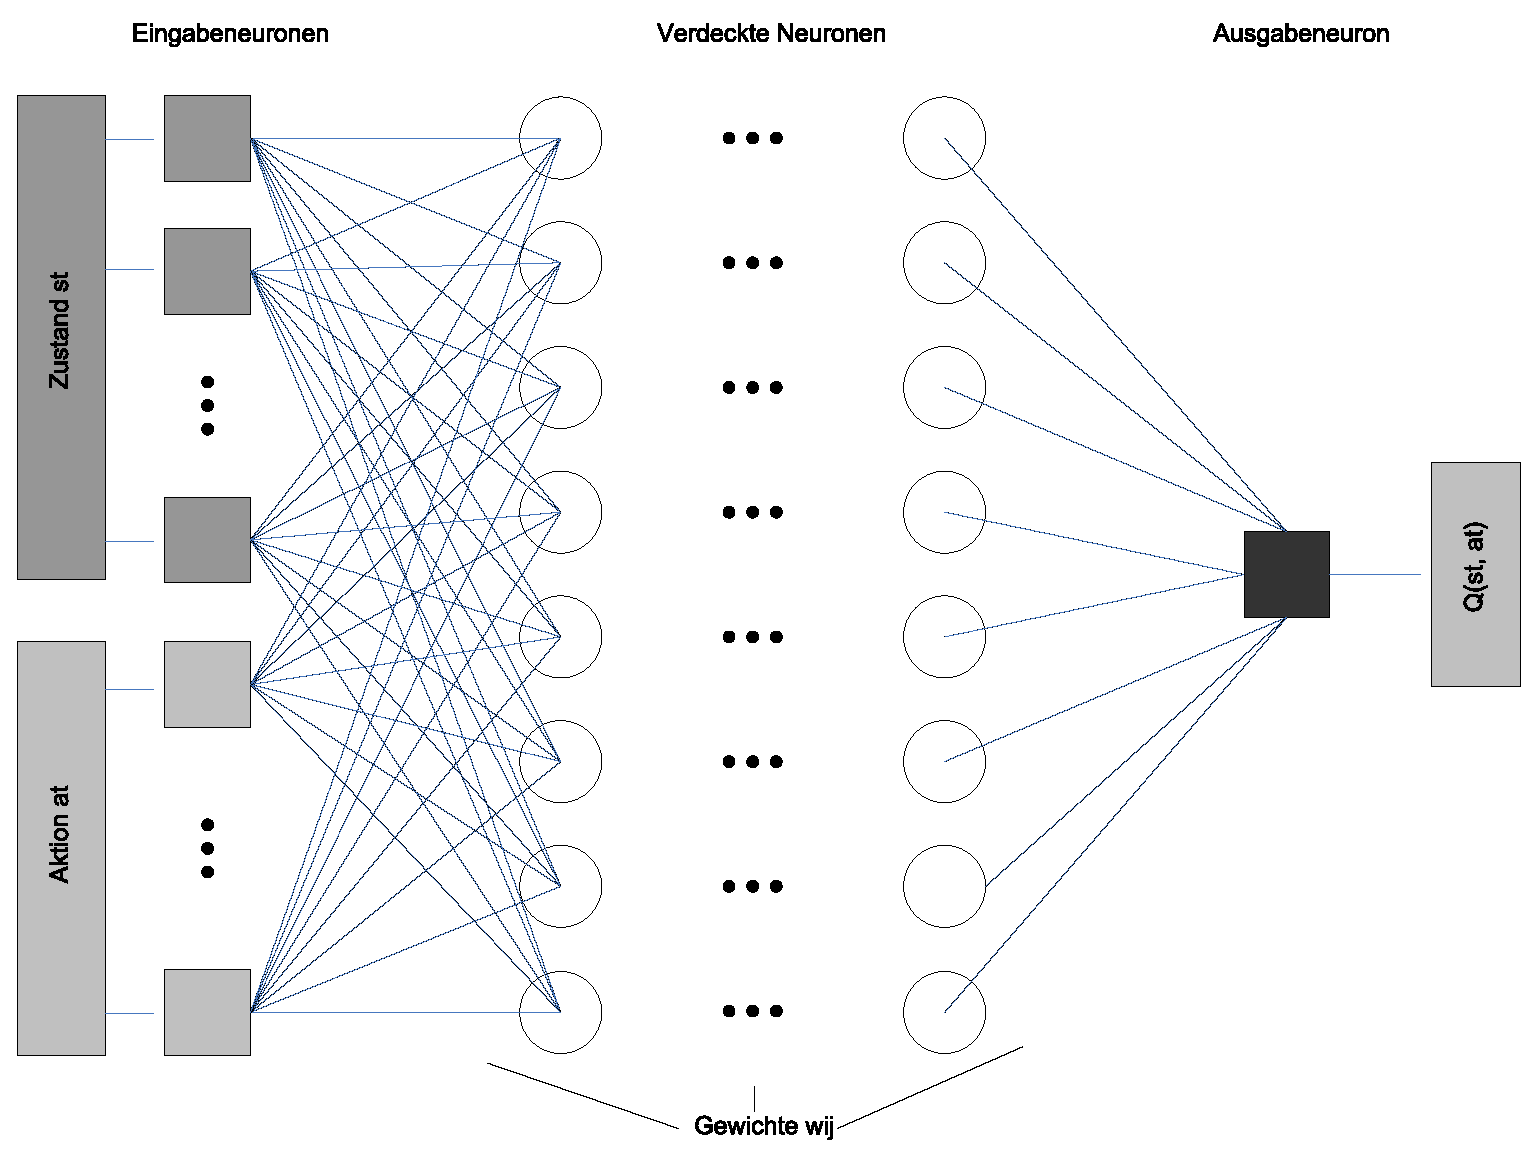
\includegraphics[width=1.00\textwidth]{../images/rl-neuronales-netz}
  \caption{Das eingesetzte neuronale Netz zur Approximation beim Q-Learning}
  \label{fig:rl-neuronales-netz}
\end{figure}

Während der Lernphase werden die gespielten Züge aufgezeichnet und anschließend
bzgl.\ der Kostenfunktion bewertet. Durch überwachtes Lernen kann das Netz diese
Bewertungen nun lernen und das neue Netz an die anderen Agenten verteilt werden.

\subsubsection{Fazit}
Es wurden die verschiedensten Fähigkeiten mittels des Reinforcement Learnings 
gelernt, die auch durchweg gute Spielleistungen erzielten. Allerdings konnten 
durch manuelle Optimierungen teilweise noch bessere Leistungen erzielt werden 
und so koexistieren im aktuellen Team sowohl manuell kodierte als auch erlernte 
Verhaltensmodule. Auffällig ist jedoch, dass im Jahr des Weltmeistertitels 
lediglich noch zwei erlernte Module im Einsatz waren - die restlichen erwiesen 
sich als nicht leistungsfähig genug.

\subsection{Middle-Size-Liga (Tribots)}
In der Middle-Size-Liga sollen allgemeine Anwendungsmethoden in der Robotik und 
der künstlichen Intelligenz wie z.\,B.\ Bildverarbeitung, Multi-Agenten-Systeme 
und Tra\-jek\-to\-ri\-en-Planung näher betrachtet werden.

Beim RoboCup-Wettbewerb treten in dieser Liga in der Regel vier mittelgroße 
Roboter, ausgestattet mit Onboard-Sensoren, auf einem Spielfeld der Größe 
12x8\,m gegeneinander an. Eine besondere Schwierigkeit stellt hier die 
durchzuführende Selbstlokalisation mittels der mitgeführten Kamera dar.

Die Roboter des "`Tribots"'-Team (s. Abbildung \ref{fig:tribots-roboter}) 
werden über ein dreirädriges Fahrwerk angetrieben und verfügen über ein 
omnidirektionales Kamerasystem sowie eine pneumatische Schusseinheit. Die 
Steuerung des Roboters wird über ein auf dem Chassis montiertes Sub-Notebook 
übernommen; die Kommunikation mit den anderen Teammitgliedern erfolgt über 
W-LAN \cite{url:Tribots2006}.

\begin{figure}
  \centering
  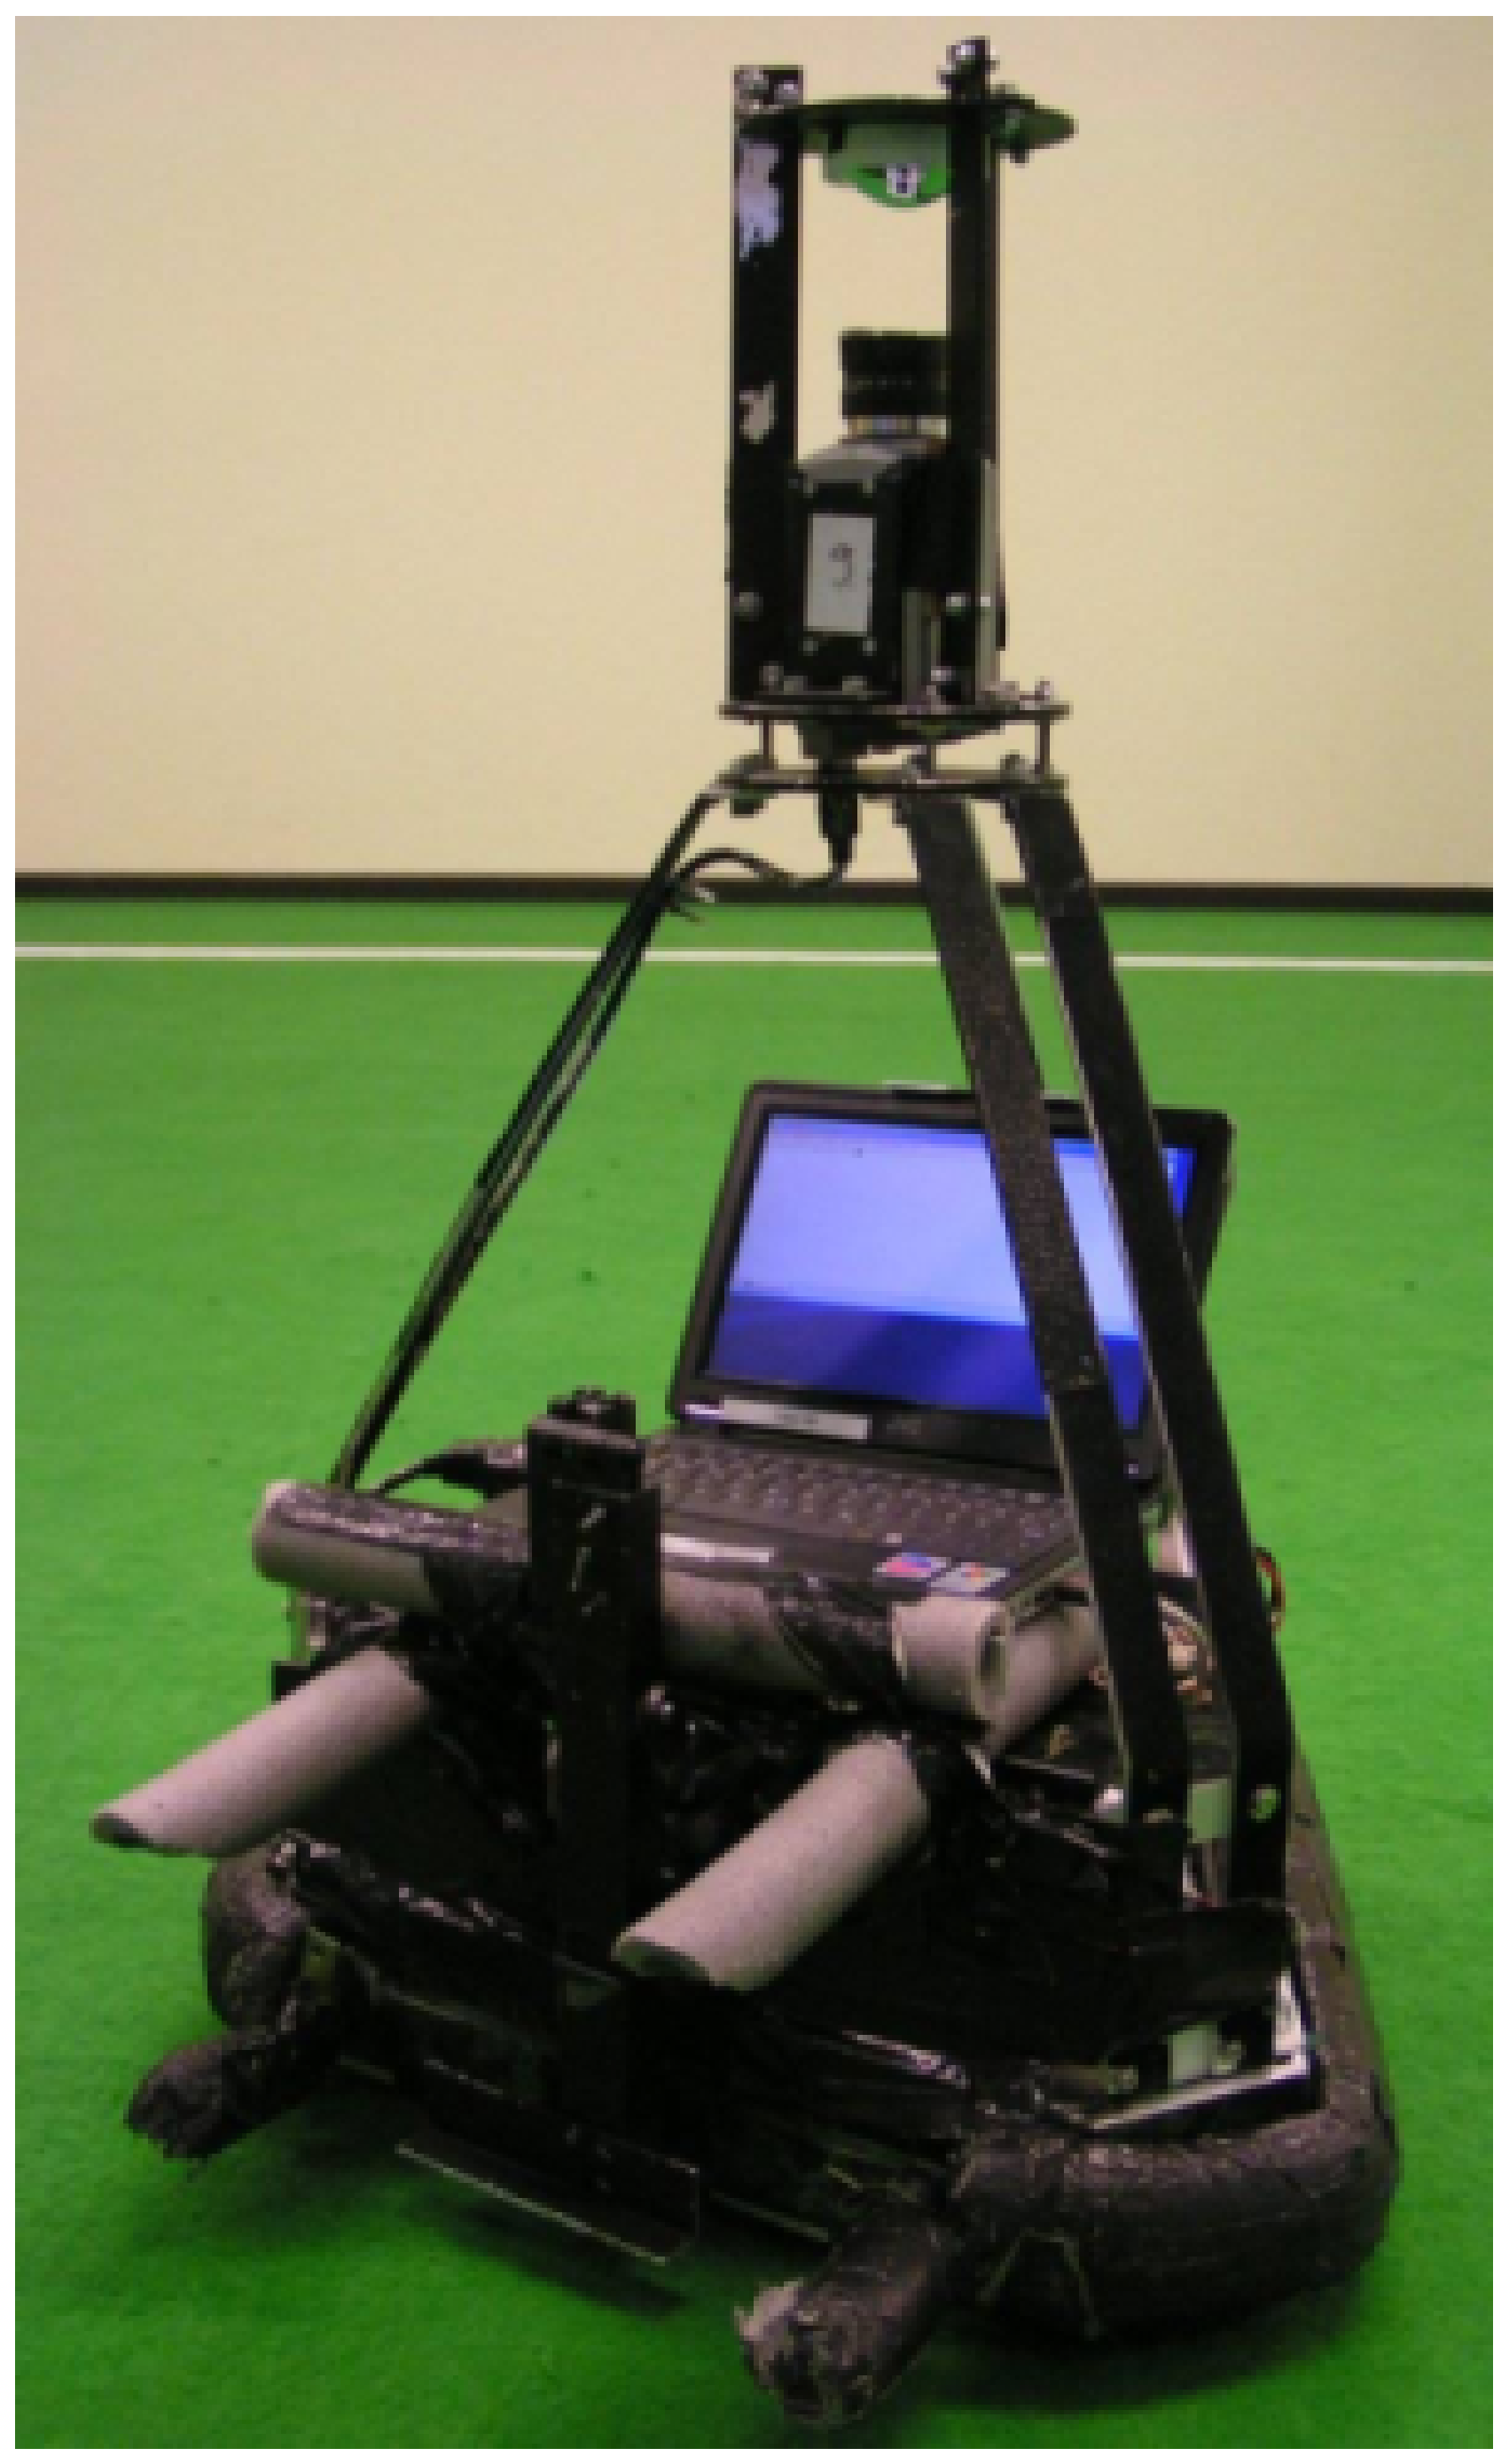
\includegraphics[width=0.40\textwidth]{../images/tribots-roboter}
  \caption{Ein Roboter des Tribots-Teams. Quelle: Webseite der Brainstormers Tribots}
  \label{fig:tribots-roboter}
\end{figure}

\subsubsection{Aufbereitung der Sensorinformationen}
Um dem Roboter ein möglichst genaues physikalisch-geometrisches Modell des 
aktuellen Spielgeschehens zur Verfügung zu stellen, werden zunächst über die 
Sensoren (omnidirektionale Kamera sowie Odometrie-Einheit) Daten der Umwelt 
gesammelt. Die zentale und wichtigste Information ist die eigene Position des 
Roboters auf dem Spielfeld. Diese wird über die von der Kamera aufgenommenen 
weißen Linien des Spielfelds bestimmt, zusätzlich werden die Daten des 
zurückgelegten Weges (Odometrie) benutzt. Allerdings sind diese beiden 
Sensorinformationen teilweise recht ungenau, weshalb kein tatsächlich exaktes 
Umweltbild ermittelt werden kann. Weiterhin muss die Ballposition und 
-geschwindigkeit sowie die Geschwindigkeit des Roboters ermittelt werden.

Ein Problem stellt die begrenzt zur Verfügung stehende Rechenkapazität dar. 
Dieser Umstand erfordert es, dass die Kamerabilder lediglich mittels eines sehr 
einfachen Farberkennungs- und Subsampling-Algorithmus verarbeitet werden, um so 
die verschiedenen Objekte anhand der Farben zuzuordnen: der Ball ist laut 
Regelwerk rot, die Tore blau und gelb sowie die Roboter schwarz. Neben der 
Erfassung des aktuellen Zustands wird außerdem über verschiedene Verfahren eine 
Vorhersage über zukünftige Parameter (also z.\,B.\ die Ballposition) getroffen.

Auf Basis des so erstellten Umweltmodells kann der Roboter nun das 
entsprechende Verhalten ausführen.

\subsubsection{Lernen von Einzelfähigkeiten}
Das Lernverfahren der Simulationsliga ist nicht direkt auf die realen Roboter 
anwendbar, da hier zu viele Lernversuche durchgeführt werden müssten. 
Stattdessen wählte man eine kombinierte Vorgehensweise: Der Lernvorgang wurde 
mit einem simulierten Roboter durchgeführt und diese Lerndaten anschließend auf 
den realen Roboter übertragen.
Am Beispiel des Verhaltens "`InterceptBall"' wird deutlich, dass die Lernaufgabe
tatsächlich nicht am realen Roboter hätte durchgeführt werden können. Denn das
mittels Q-Learning erlernte Verhalten benötigte 10 Mio. Iterationen, was einer
Realzeit von etwa 916 Std. entspräche.

Obwohl die so gelernten Verhalten auf dem realen Roboter die gewünschte Aktion
durchführen, bleibt das Problem, dass die optimale Eigenschaft durch die
Übertragung von Simulation auf Realität verloren geht. Aus diesem Grunde wurde
von den Verantwortlichen ein modifizierter Q-Learning-Algorithmus, die Neural
Fitted Q-Iteration, eingeführt. Dieses Verfahren erlaubt das Training direkt am
realen Roboter mit deutlich verringerter Interaktionszeit.

\subsubsection{Lernen von Regelungsaufgaben}
Von großer Bedeutung für einen mobilen Roboter ist die Fahrwerkssteuerung, da 
die erforderlichen Fahrtbewegungen (Richtung und Geschwindigkeit) möglichst 
präzise und schnell durchgeführt werden müssen.

Für die aktuelle Sollgeschwindigkeit wird für jeden einzelnen Motor eine 
separate Geschwindigkeit berechnet und der Motor entsprechend geregelt. 
Problematisch wird dies allerdings durch verschiedene Einflussfaktoren, wie 
z.\,B.\ die entstehende Reibung. Ausgehend von diesem Problem lässt sich das 
Verhalten des Geschwindigkeitsreglers auch mittels Reinforcement Learning 
lernen und somit optimieren.

\subsection{Fazit}
Die Erfahrungen mit Reinforcement Learning des Osnabrücker RoboCup-Teams waren 
i.\,A.\ positiv und die Qualität der gelernten Module überstieg anfangs jeweils 
die des handcodierten Pendants. Durch die gewonnenen Erkenntnisse beim Einsatz 
des Verstärkungslernens konnten einige der Module daraufhin optimiert werden, 
sodass letztlich doch eine handcodierte, minimal leistungsfähigere Variante in 
den Wettkämpfen zum Einsatz kommt.

Gerade diese Rückkopplung und die Kombination klassischer und erlernter Module 
werden als zukunftsfähig angesehen, u.\,a.\ in industriellen Anwendungen wie 
der Regelungstechnik oder reaktivem Scheduling.

%%%
%%% Anhaenge: Glossar, Bibliographie...
%%%

%\cleardoublepage % oder \clearpage
%\phantomsection 

%\appendix
%\pdfbookmark[-1]{\appendixname}{\appendixname} 

%%% Bibliographie-Stil
% abbrvdin, alphadin, plaindin, unsrtdin
\bibliographystyle{alphadin}

%%% Anstatt 'Literatur' -> 'Quellen'
\renewcommand{\bibname}{Quellen}

%%% Bibliographie ausgeben
\bibliography{../Literatur}

%%% Glossar ausgeben
%\printgloss{Glossar}

\end{document}
%%% END OF FILE